%%%%%%%%%%%%%%%%%%%%%%%%%%%%%%%%%%%%%%%%%%%%%%%%%%%%%%%%%%%%
%%  This Beamer template was created by Cameron Bracken.
%%  Anyone can freely use or modify it for any purpose
%%  without attribution.
%%
%%  Last Modified: January 9, 2009
%%

\documentclass[xcolor=x11names,compress]{beamer}
\usepackage[utf8]{inputenc} 
\usepackage[T1]{fontenc}
\usepackage{cmbright}

%% General document %%%%%%%%%%%%%%%%%%%%%%%%%%%%%%%%%%
\usepackage{graphicx}
\usepackage{tikz}

\usepackage[style=authoryear]{biblatex}
\usetikzlibrary{decorations.fractals}
%%%%%%%%%%%%%%%%%%%%%%%%%%%%%%%%%%%%%%%%%%%%%%%%%%%%%%


%% Beamer Layout %%%%%%%%%%%%%%%%%%%%%%%%%%%%%%%%%%
\useoutertheme[subsection=false,shadow]{miniframes}
\setbeamerfont{title like}{shape=\scshape}
\setbeamerfont{frametitle}{shape=\scshape}

\setbeamercolor*{lower separation line head}{bg=DeepSkyBlue4} 
\setbeamercolor*{normal text}{fg=black,bg=white} 
\setbeamercolor*{alerted text}{fg=red} 
\setbeamercolor*{example text}{fg=black} 
\setbeamercolor*{structure}{fg=black} 

 \usenavigationsymbolstemplate{}
\setbeamercolor*{palette tertiary}{fg=black,bg=black!10} 
\setbeamercolor*{palette quaternary}{fg=black,bg=black!10} 

\renewcommand{\(}{\begin{columns}}
\renewcommand{\)}{\end{columns}}
\newcommand{\<}[1]{\begin{column}{#1}}
\renewcommand{\>}{\end{column}}
%%%%%%%%%%%%%%%%%%%%%%%%%%%%%%%%%%%%%%%%%%%%%%%%%%
\useoutertheme{infolines} % authors, etc.
%%%%%%%%%%%%%%%%%%%%%%%%%%%%%%%%%%%%%%%%%%%%%%%%%%

\bibliography{presentation.bib}

\DeclareGraphicsExtensions{.pdf,.png,.jpg, .eps}

\usepackage{color, colortbl}  
\definecolor{LightCyan}{rgb}{0.88,0.8,1}
\begin{document}


%%%%%%%%%%%%%%%%%%%%%%%%%%%%%%%%%%%%%%%%%%%%%%%%%%%%%%
\title[Compton]{Compton scattering}
%\subtitle{SUBTITLE}
\author{
	Friedrich Schüßler, Volker Karle\\
}
\institute% (optional)
{ \inst{}%
    University of Freiburg
  \and
  \inst{}%
    Assistant: Kilian Rosbach}
\date{\today}

\frame{\titlepage}
%%%%%%%%%%%%%%%%%%%%%%%%%%%%%%%%%%%%%%%%%%%%%%%%%%%%%%

\begin{frame}{Inhaltsverzeichnis}
\tableofcontents
\end{frame}

\section{Theoretische Grundlagen}
\begin{frame}[t]{Compton Streuung -- Energieerhaltung}
\begin{figure}[htpb]
    \centering
    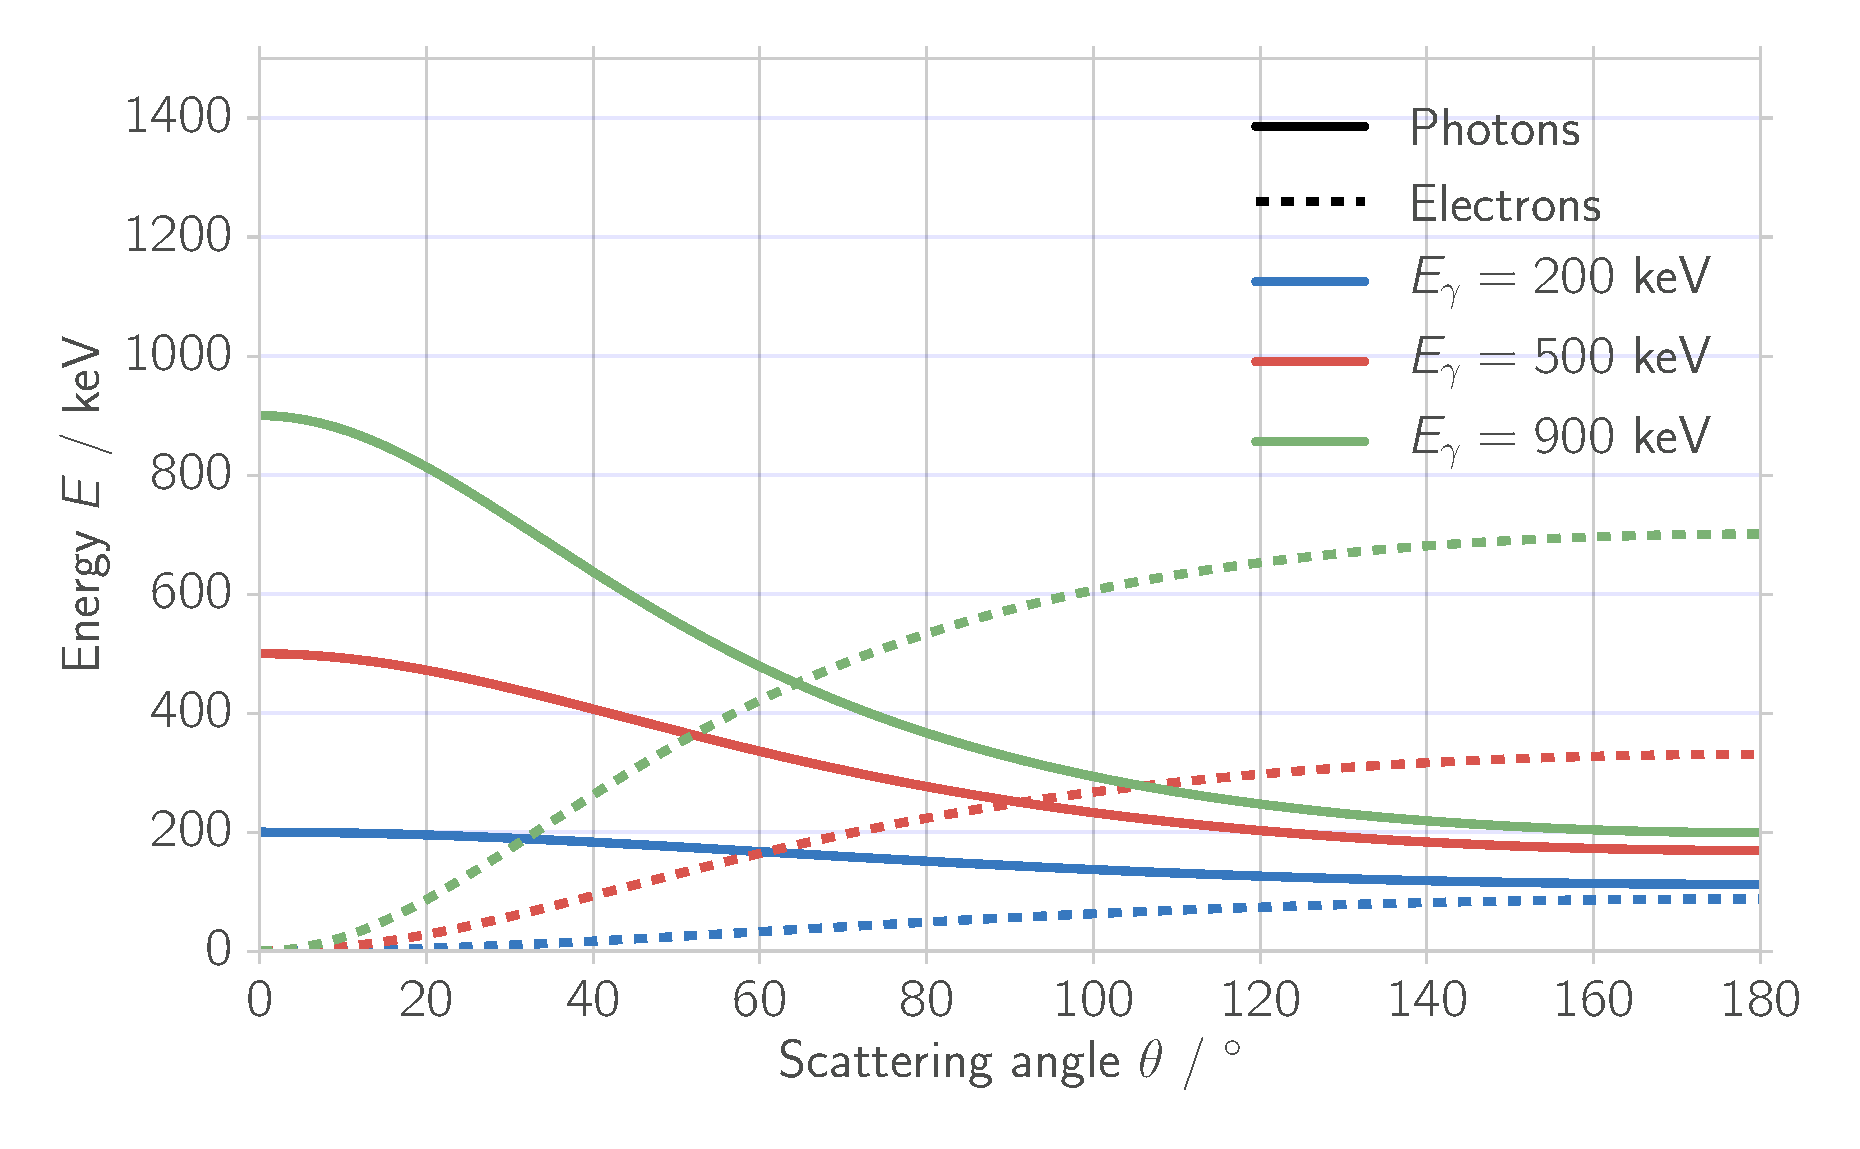
\includegraphics[width=1.0\linewidth]{../analysis/figures/theory_conservation}
\label{fig:theory_cons}
\end{figure}
\end{frame}

\begin{frame}[t]{Compton Streuung -- Diff. Wirkungsquerschnitt}
\begin{figure}[htpb]
    \centering
    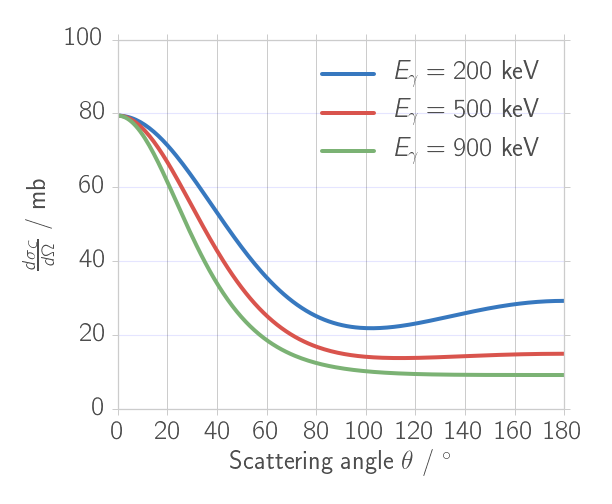
\includegraphics[width=1.0\linewidth]{../analysis/figures/theory_diff_cs}
\label{fig:theory_diff}
\end{figure}
\end{frame}

\section{Experimenteller Aufbau}
\begin{frame}[t]{Aufbau ohne Elektronik}
\begin{figure}[htpb]
    \centering
    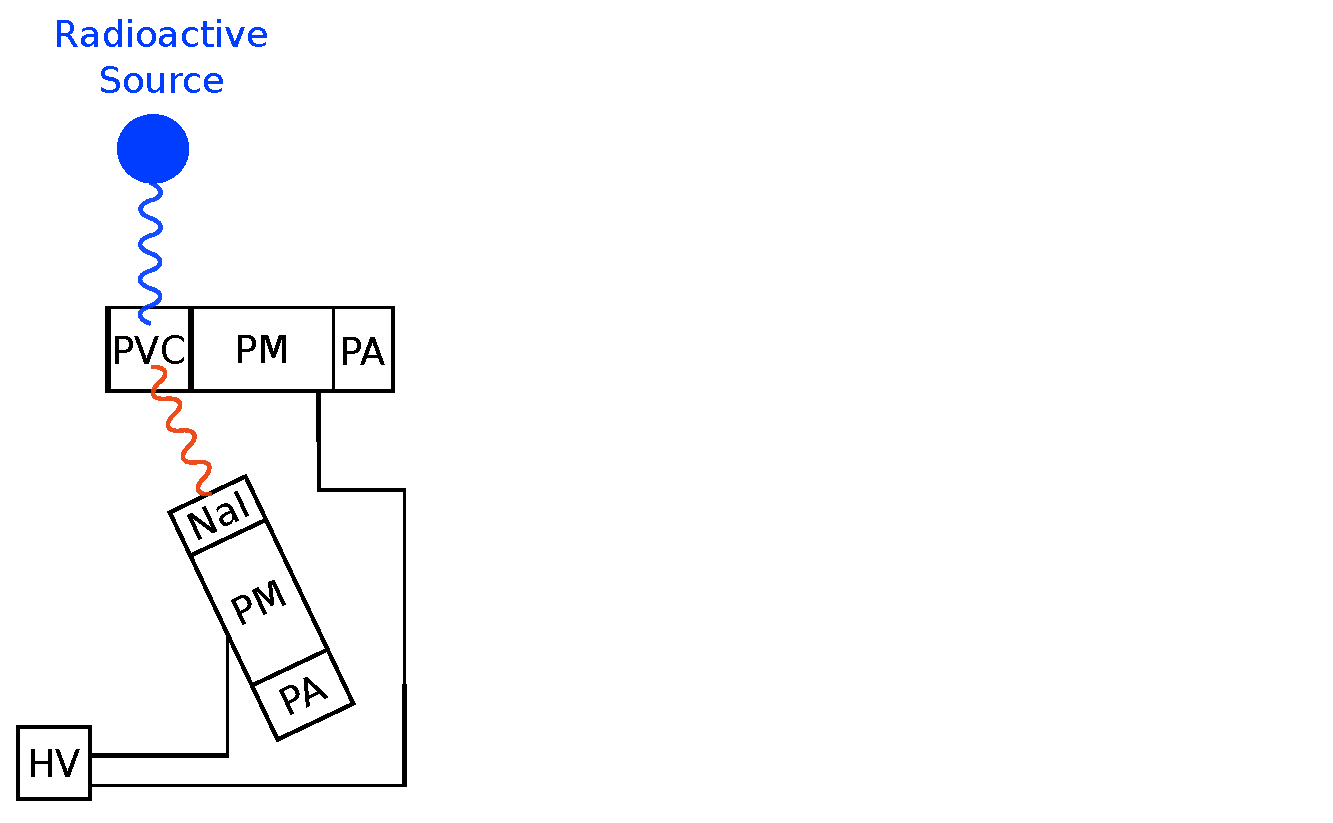
\includegraphics[width=1.0\linewidth]{../figures/setup_pres_pre}
\label{fig:setup_pre}
\end{figure}
\end{frame}

\begin{frame}[t]{Aufbau mit Elektronik}
 \begin{figure}[htpb]
    \centering
    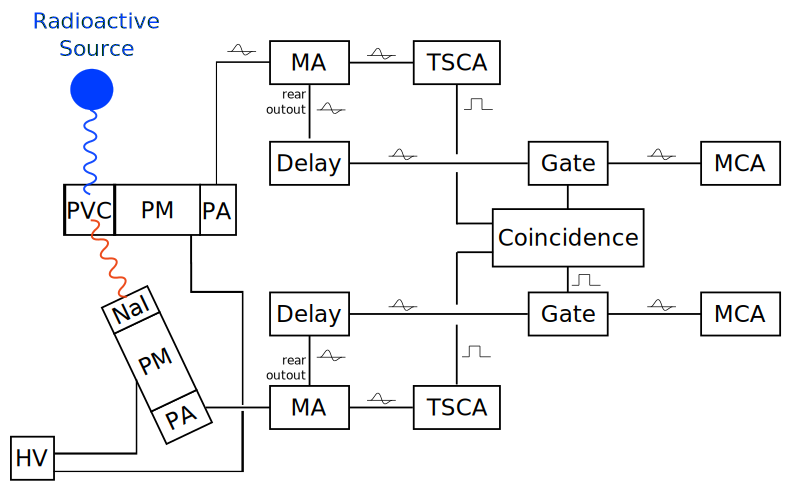
\includegraphics[width=1.0\linewidth]{../figures/setup_pres}
\label{fig:setup_pre}
\end{figure}
\end{frame}

\subsection{$^{137}$Cs und  $^{22}$Na}
\begin{frame}[t]{Zerfallsschemata von $^{137}$Cs und  $^{22}$Na}
 \begin{figure}[htpb]
    \centering
    %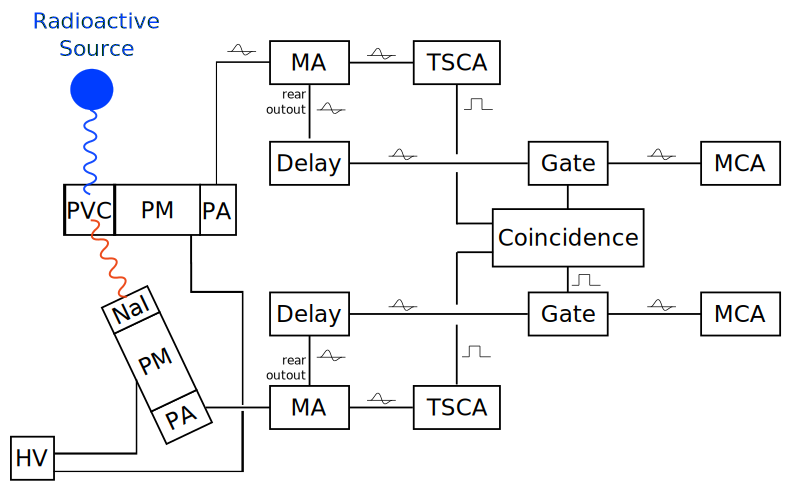
\includegraphics[width=1.0\linewidth]{../figures/setup_pres}
    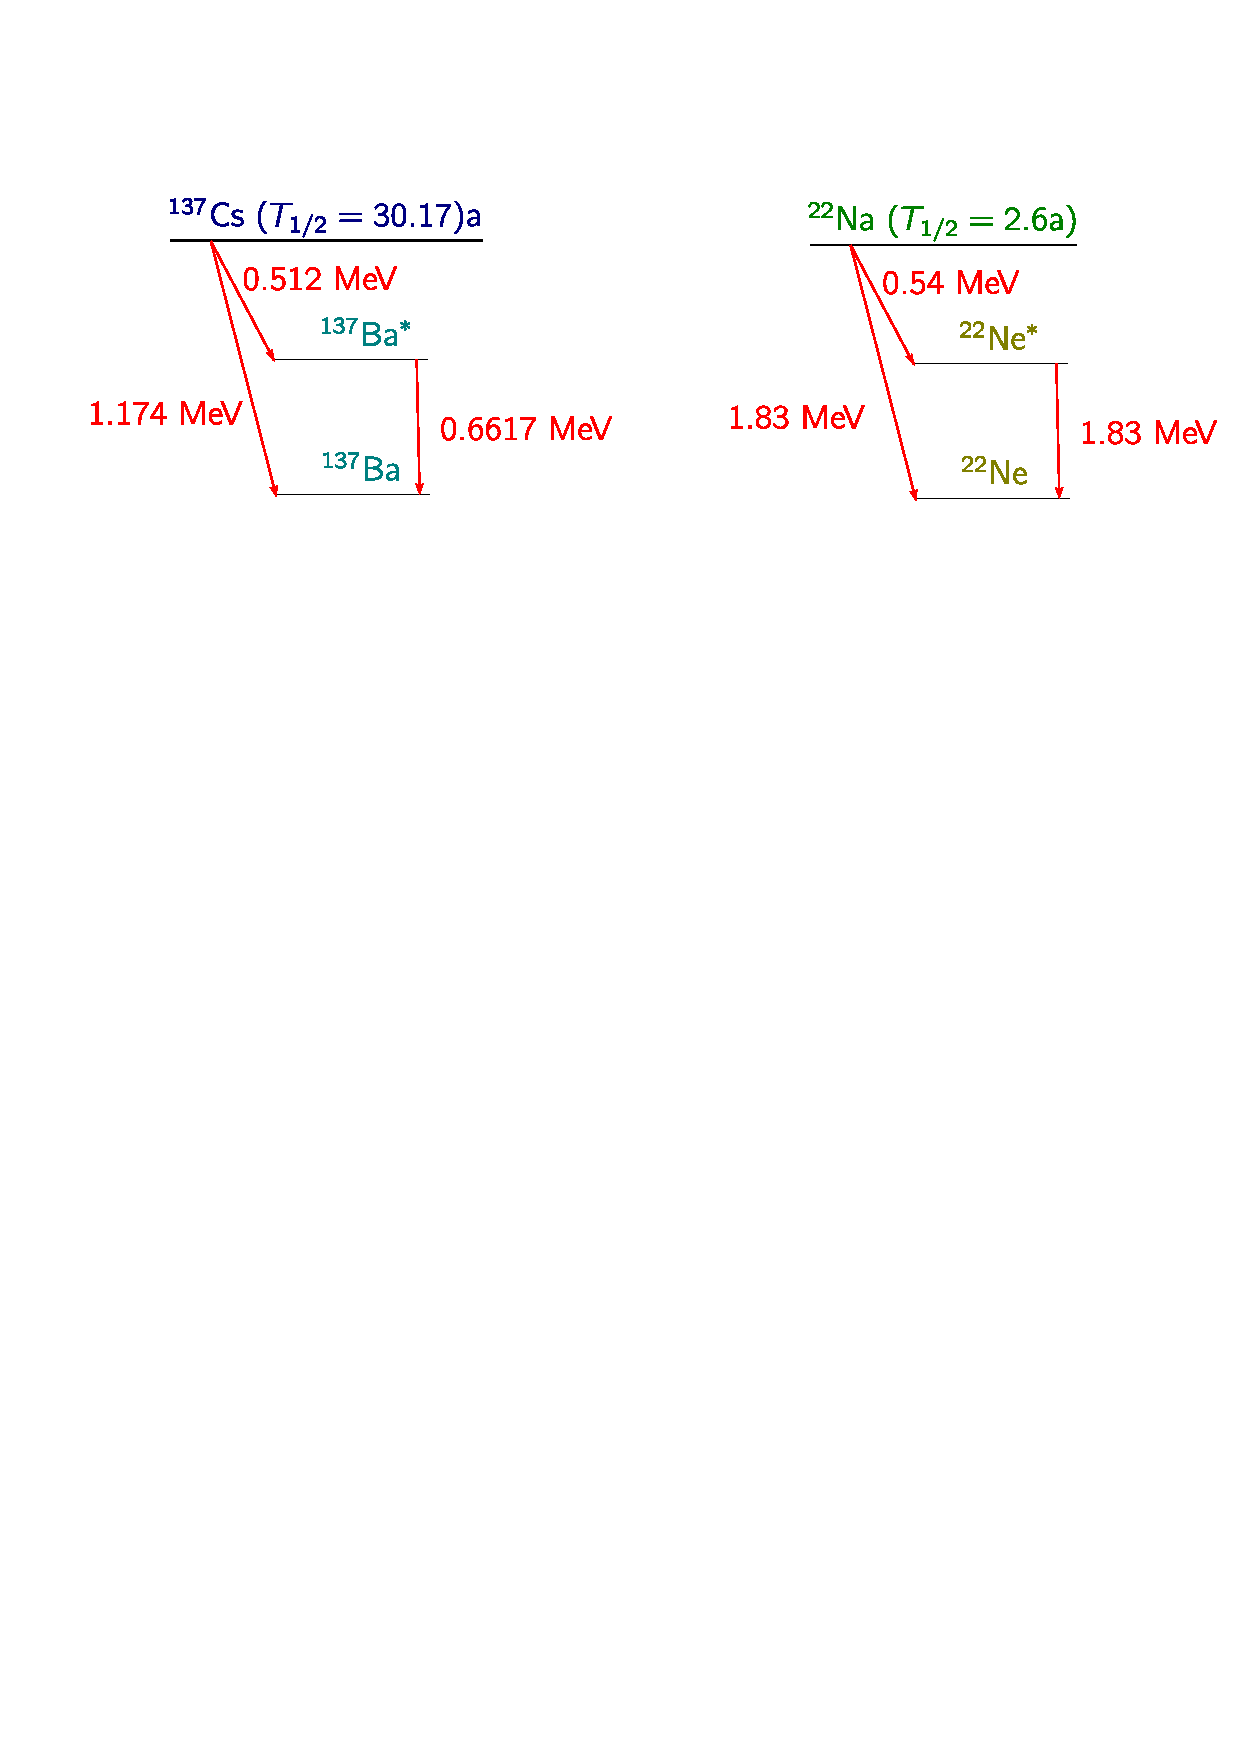
\includegraphics[width=1.0\linewidth]{../figures/terms}
\label{fig:term_schemata}
\end{figure}
\end{frame}

\subsection{Szintillisatoren}
\begin{frame}[t]{Sichtbare Peaks und Kanten für beide Szintillisatoren}
\begin{table}[htpb]
    \centering
    \label{tab:mono_calibration}
    \begin{tabular}{l l r c c}
        \rowcolor{LightCyan} Probe & Peak/Kante & $E$ / keV& NaI Szinti & PCV Szinti \\
        \cellcolor{LightCyan}$^{137}$Cs & Photo & 662 & sichtbar &  \\
        \cellcolor{LightCyan} & Compton& 477& sichtbar  &  sichtbar  \\
        \cellcolor{LightCyan} & Rückstreu& 183&  sichtbar &  \\
        \cellcolor{LightCyan}$^{22}$Na & Photo& 511& sichtbar  &  \\
        \cellcolor{LightCyan} & Compton& 341& sichtbar  & sichtbar  \\
        \cellcolor{LightCyan} & Photo& 1277& sichtbar  & \\
        \cellcolor{LightCyan} & Compton& 1064& sichtbar  & sichtbar \\
    \end{tabular}
\end{table}
\end{frame}


\section{Calibration of PS scintillator}
\begin{frame}[t]{$^{22}$Na sample (measurement time 16.5h) }
\begin{figure}[htpb]
    \centering
    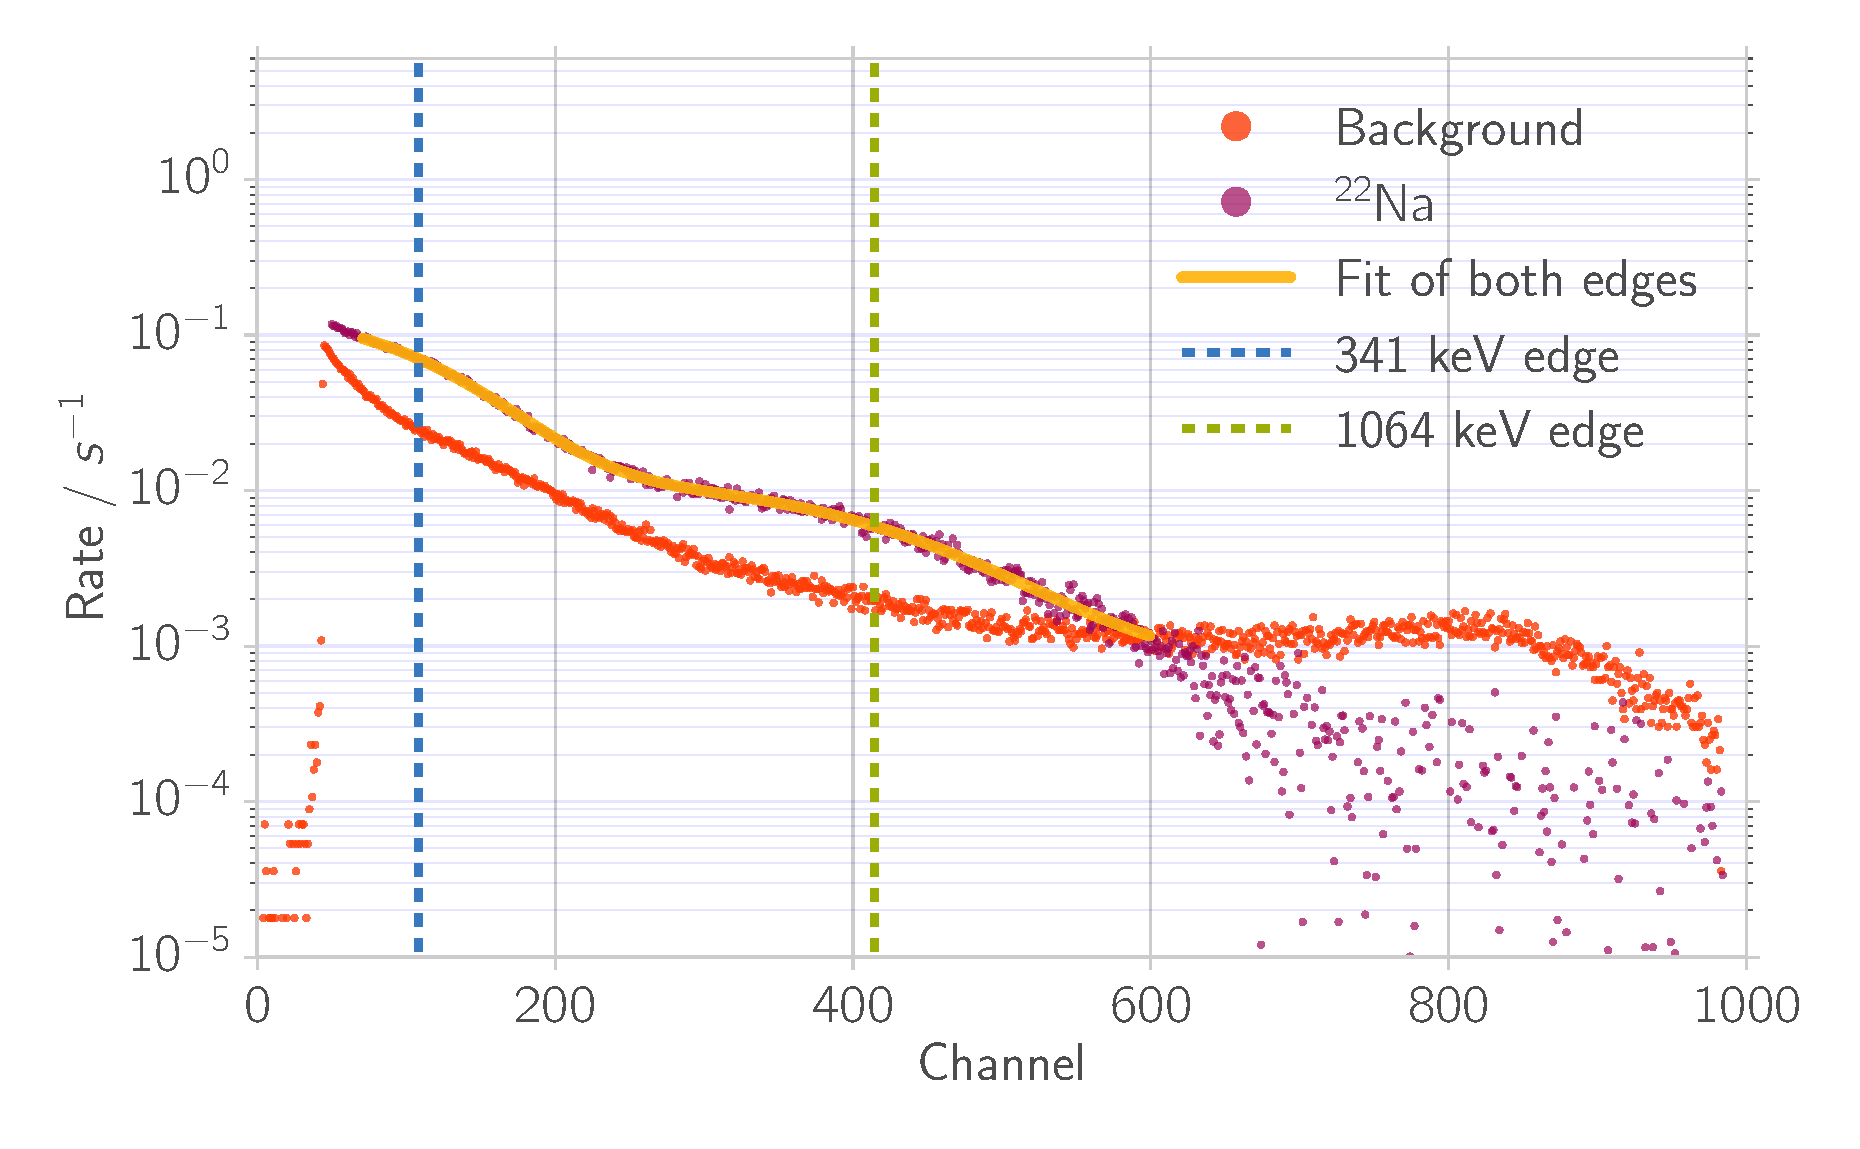
\includegraphics[width=1.0\linewidth]{../analysis/figures/calib_ps_na}
\label{fig:calib_ps_na}
\end{figure}
\end{frame}

\begin{frame}[t]{$^{137}$Cs sample (measurement time 6h) }
\begin{figure}[htpb]
\centering
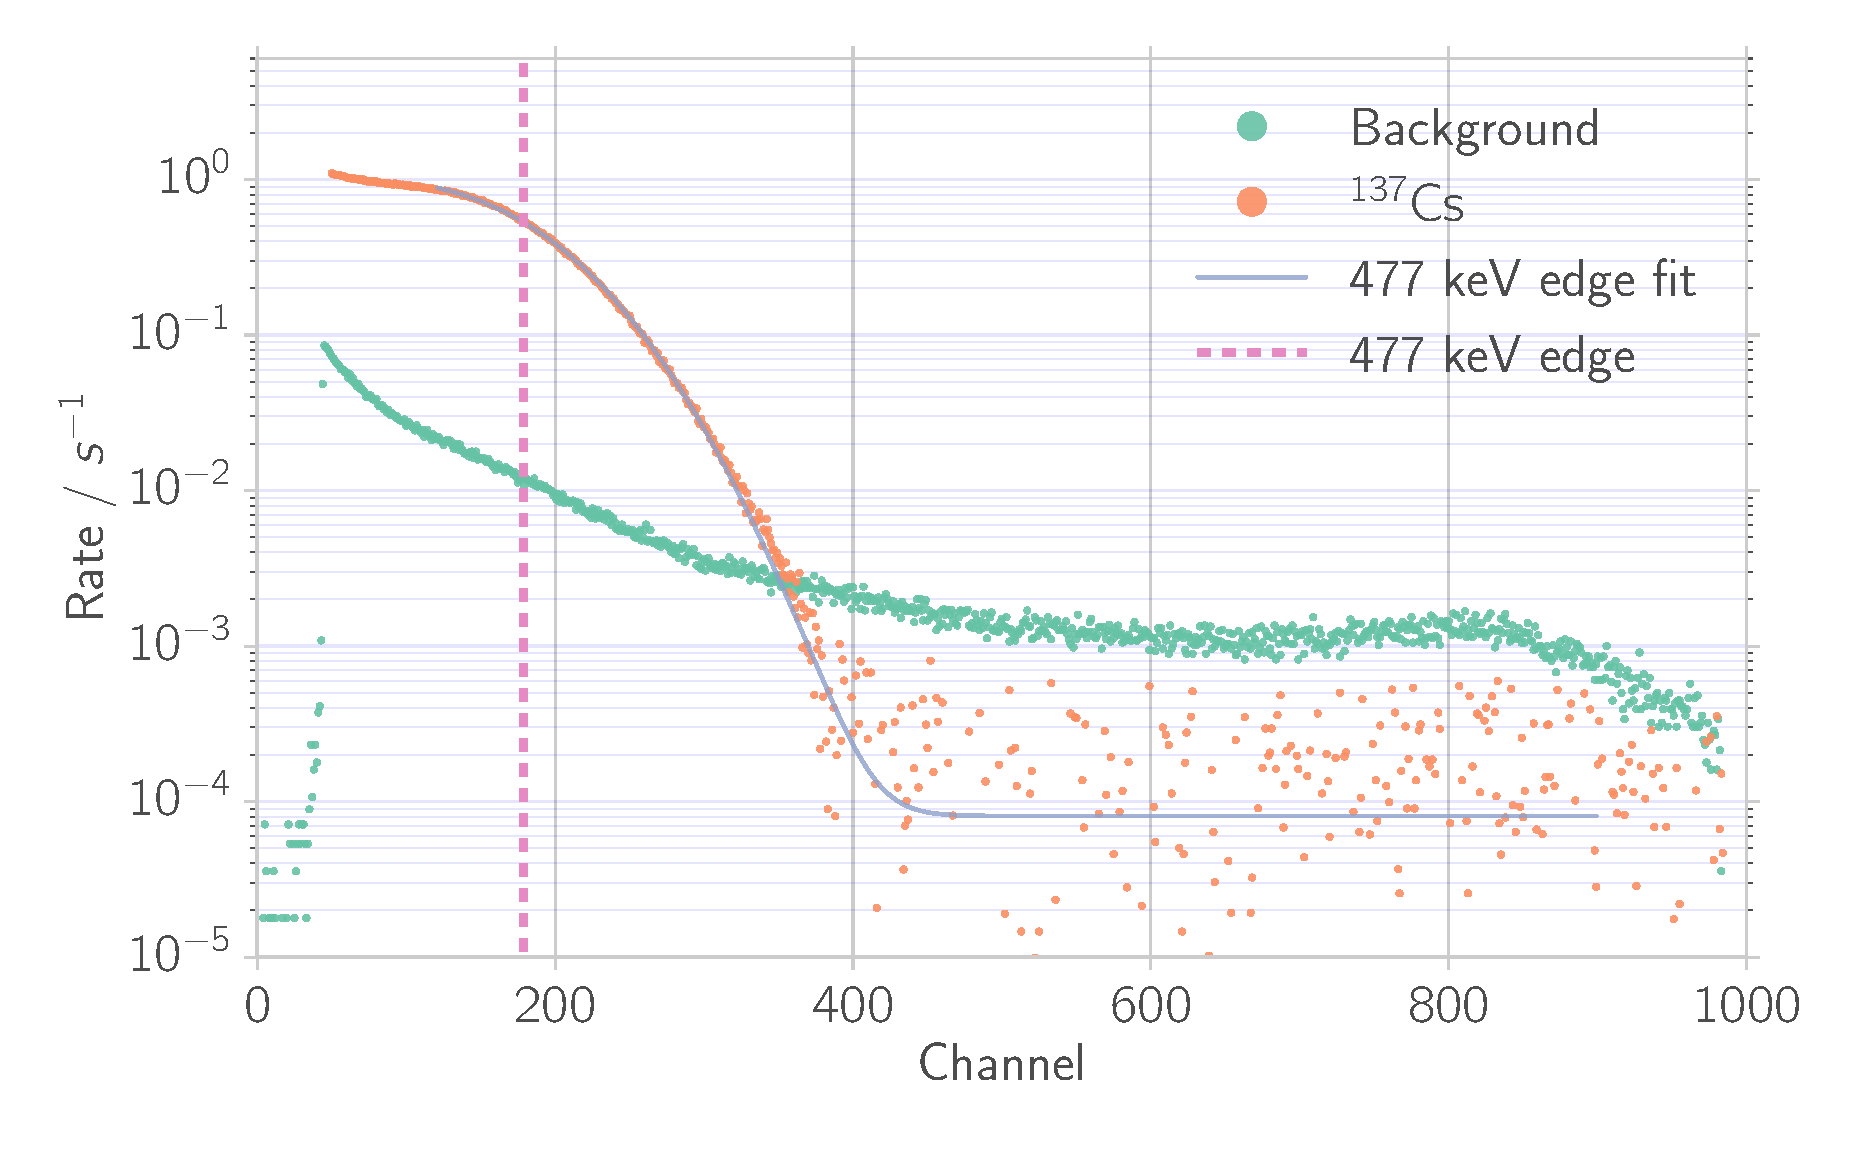
\includegraphics[width=1.0\linewidth]{../analysis/figures/calib_ps_cs}
\label{fig:calib_ps_cs}
\end{figure}
\end{frame}

\begin{frame}[t]{Linear fit}
\begin{figure}[htpb]
    \centering
    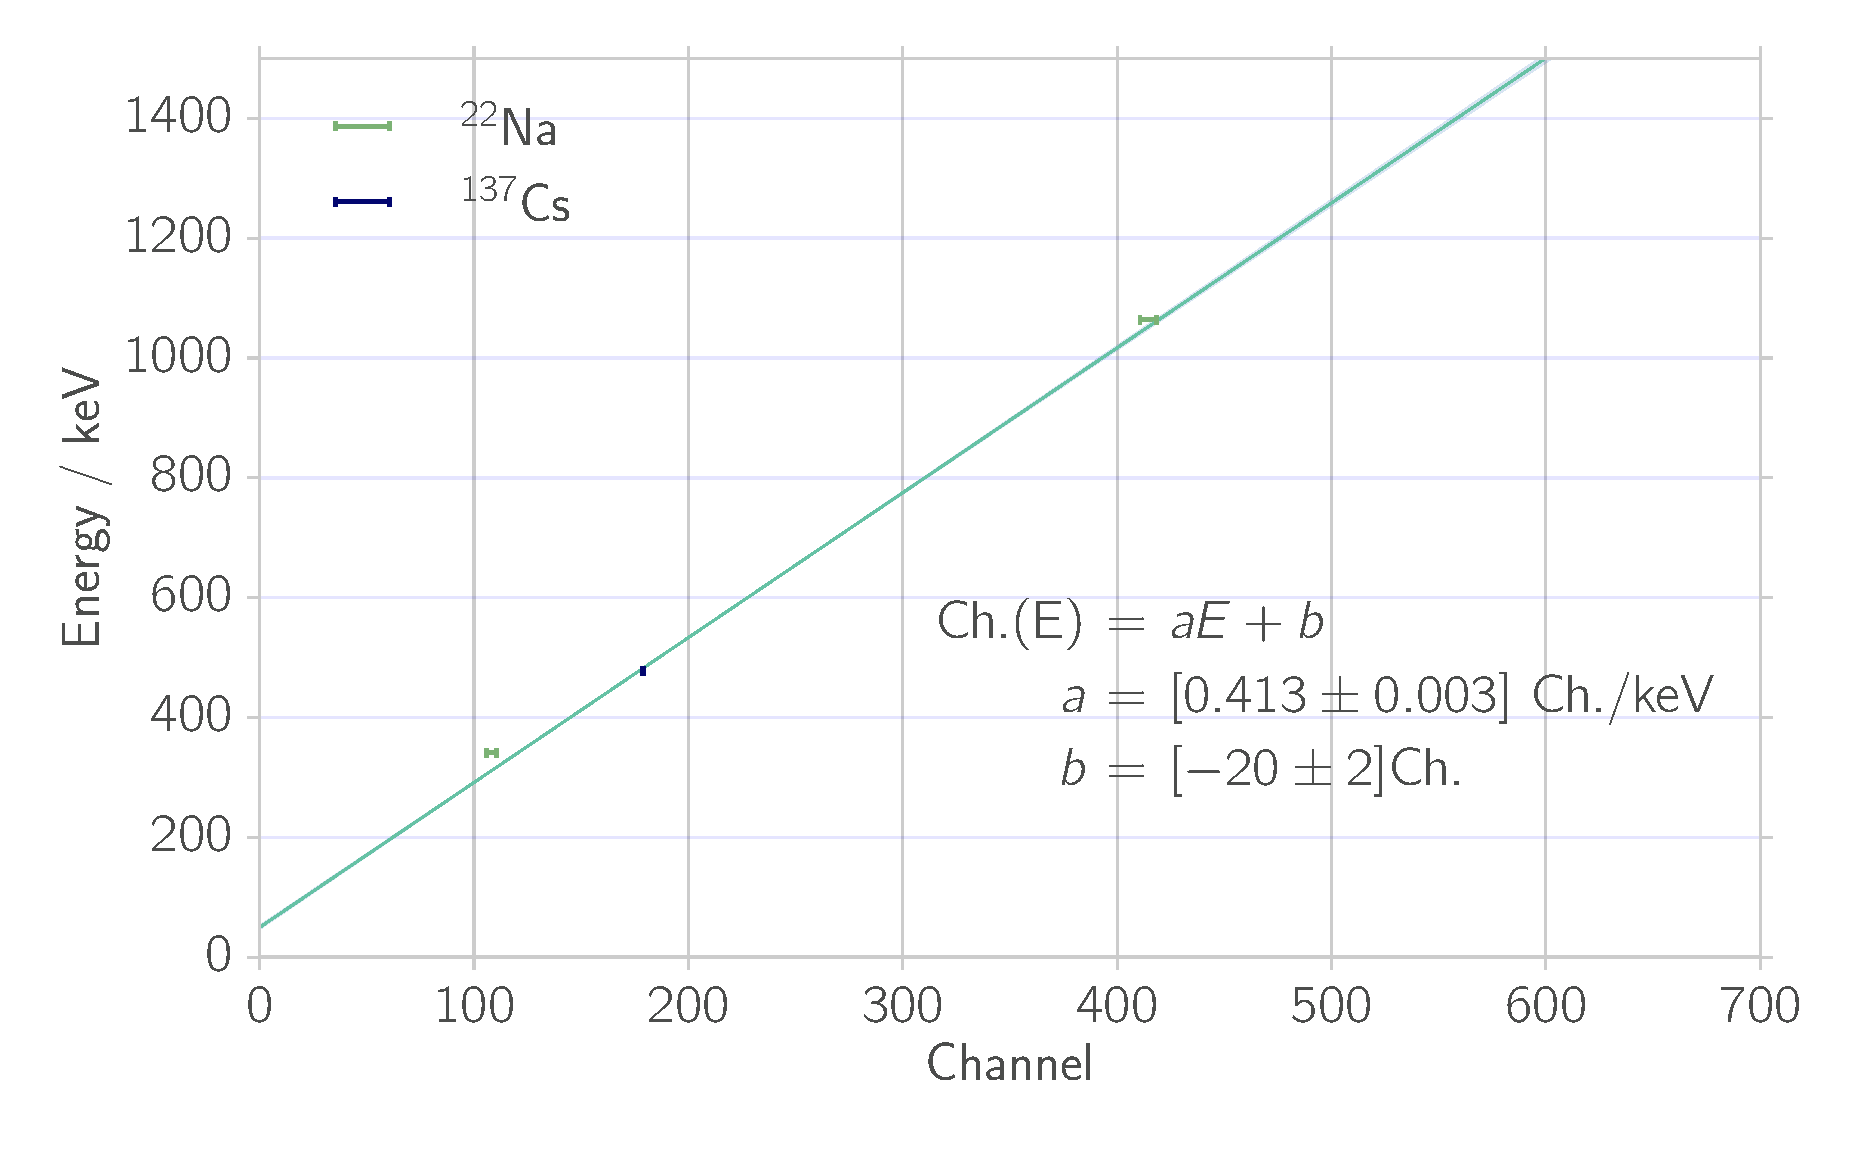
\includegraphics[width=1.0\linewidth]{../analysis/figures/calibration_ps_linear_fit}
\label{fig:calibration_ps_linear_fit}
\end{figure}
\end{frame}

\section{Calibration of Na scintillator}

\begin{frame}[t]{Peaks and fitting results of $^{137}$Cs}

    \begin{table}[htpb]
    \centering
\label{tab:peaks_cs_ps}
    \begin{tabular}{lll}
        \rowcolor{LightCyan} Name &Energy & Channel \\ 
        Photo peak & 662 keV & $8040.59 \pm 0.03$\\ 
        Compton edge & 477 keV & $5720 \pm 4$\\  
        Escape peak & 183 keV & $2510 \pm 12$
    \end{tabular}
\end{table}

\end{frame}

\begin{frame}[t]{$^{137}$Cs sample (measurement time 2.7h)}
 \begin{figure}[htpb]
    \centering
    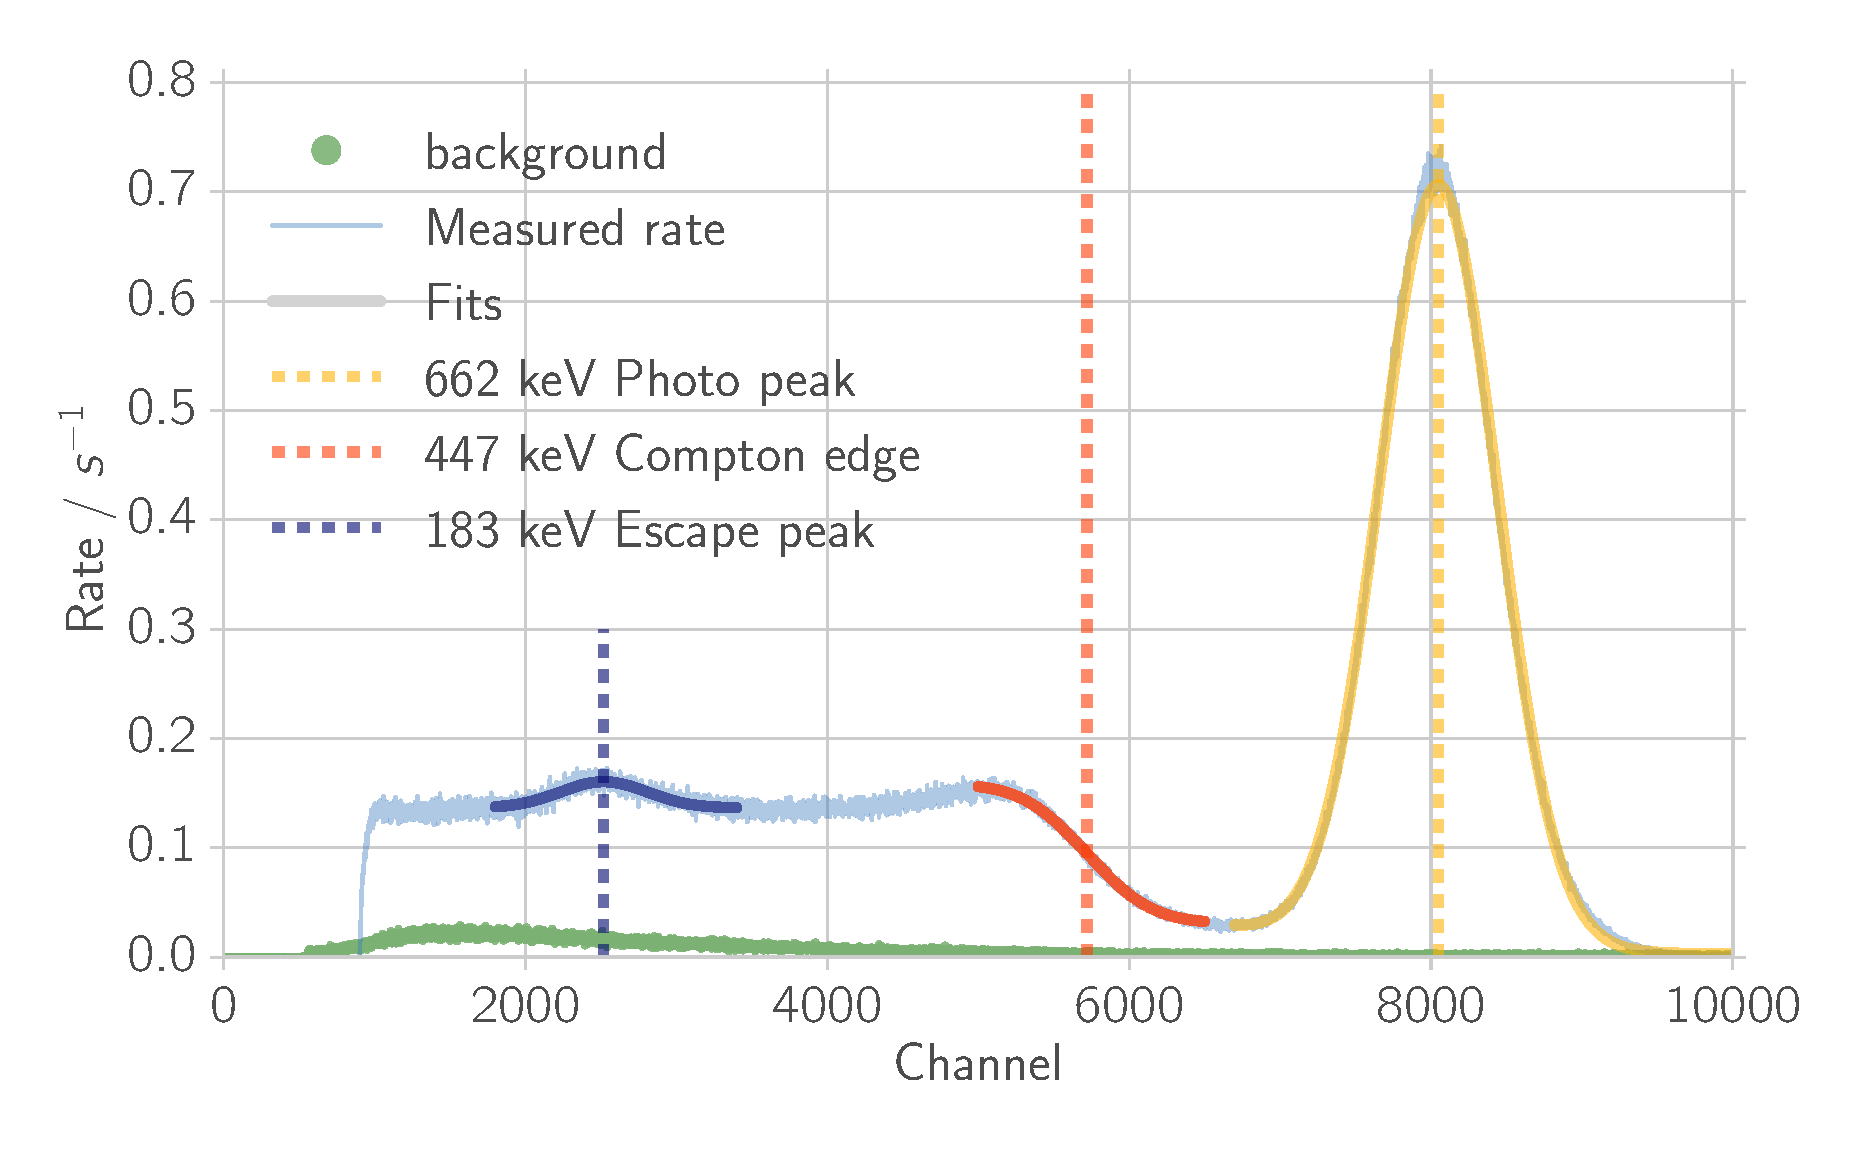
\includegraphics[width=1.0\linewidth]{../analysis/figures/histo_na_137cs}
    \label{fig:histo_na_137cs}
\end{figure}
\end{frame}

\begin{frame}[t]{Peaks and fitting results of $^{22}$Na}
    \begin{table}[htpb]
    \centering
\label{tab:peaks_na_ps}
\begin{tabular}{lll}
    \rowcolor{LightCyan} Name &Energy & Channel \\ 
       1. Photo peak& 511 keV & $6347 \pm 3$ \\ 
       2. Photo peak& 1277 keV & $14180 \pm 20 $\\
       1. Compton edge& 341 keV& $4000 \pm 2000$\\
       2. Compton edge& 1064 keV & $12000 \pm 4000$
    \end{tabular}
    \end{table}
\end{frame}

\begin{frame}[t]{$^{22}$Na sample (measurement time about 1h) }
    
\begin{figure}[htpb]
    \centering
    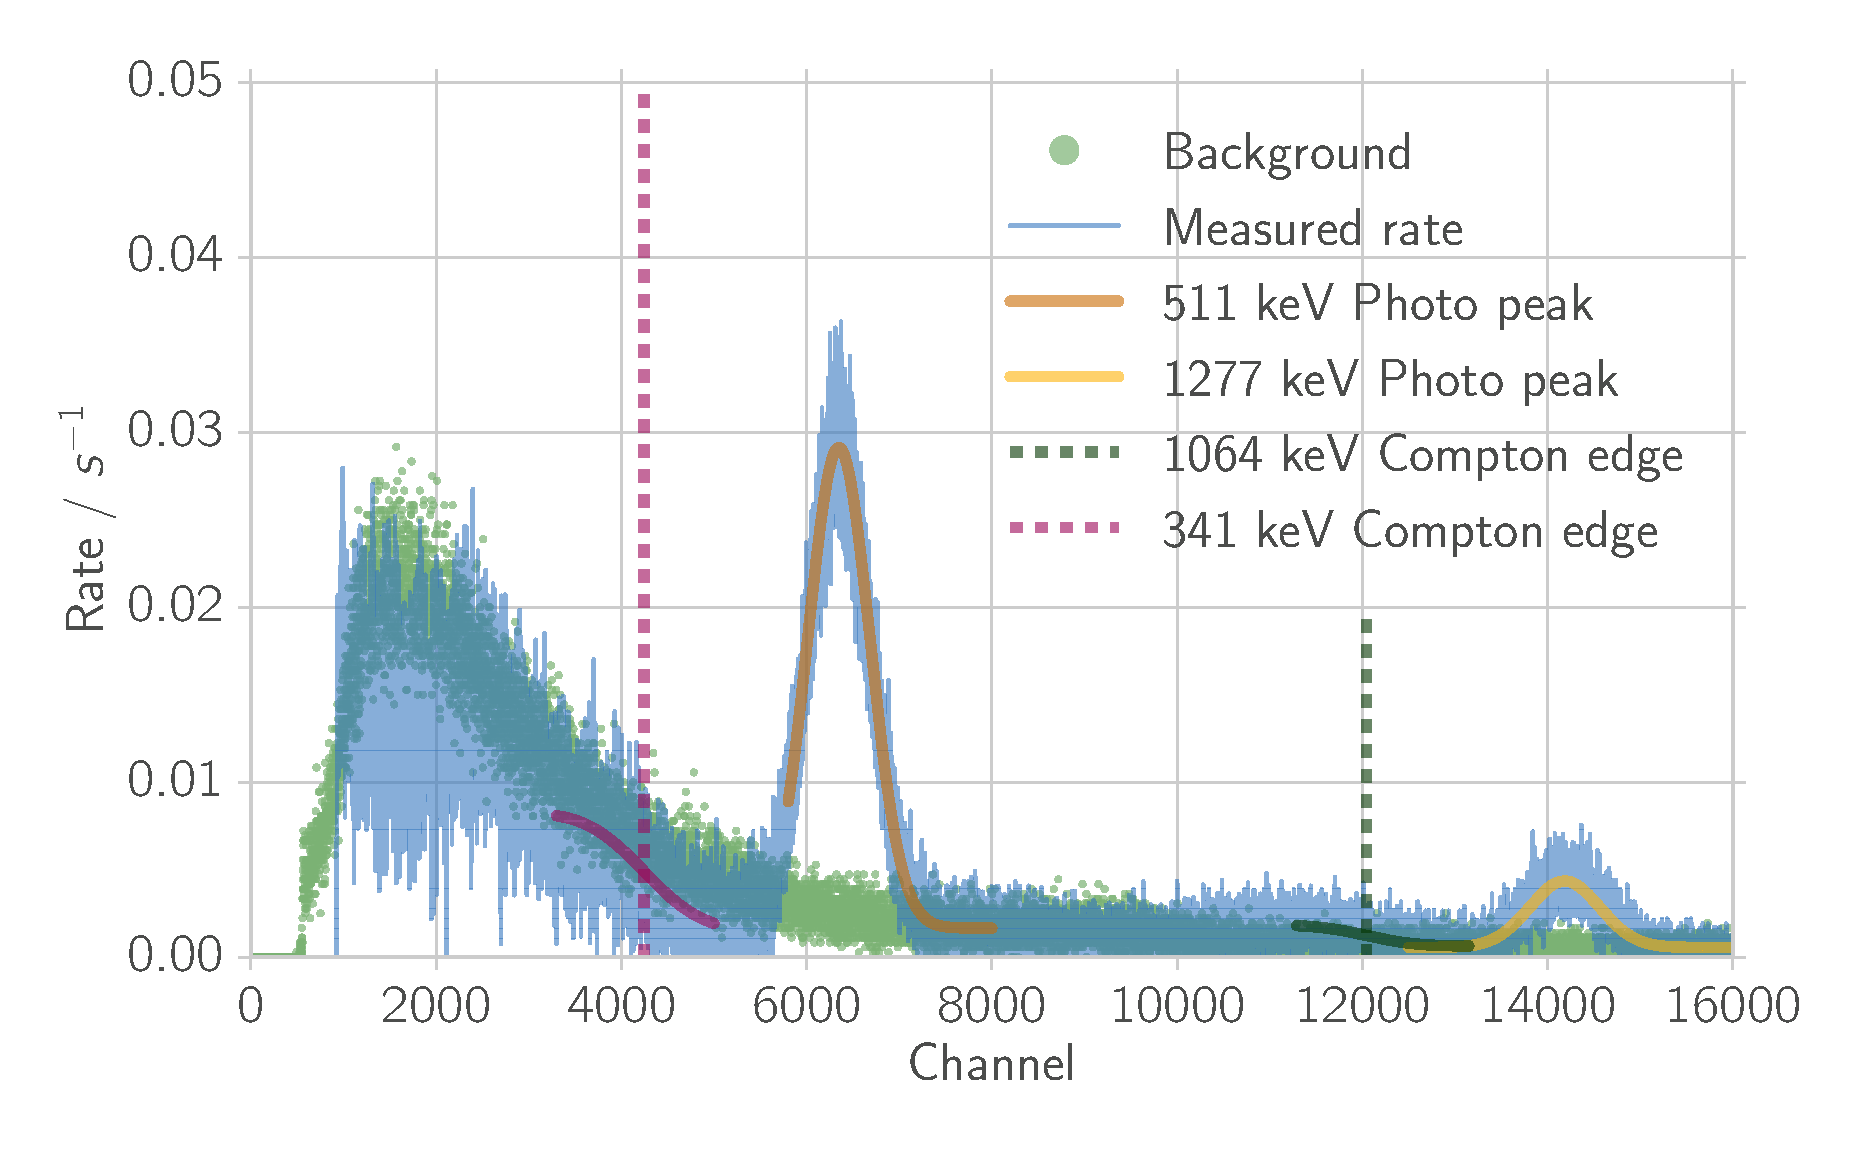
\includegraphics[width=1.0\linewidth]{../analysis/figures/histo_na_22na}
\label{fig:histo_na_22na}
\end{figure}

\end{frame}

\begin{frame}[t]{Linear fit}
 \begin{figure}[htpb]
    \centering
    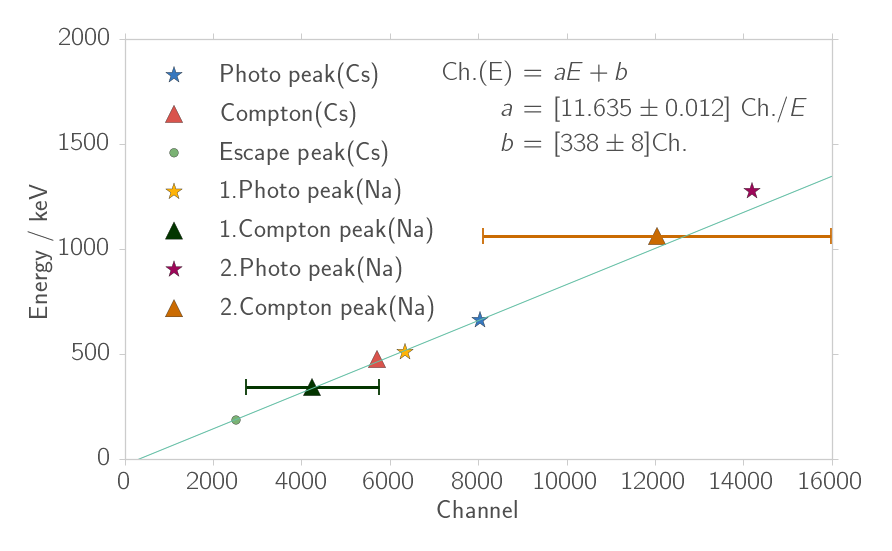
\includegraphics[width=1.0\linewidth]{../analysis/figures/calibration_na_linear_fit}
    \label{fig:calibration_na_linear_fit}
\end{figure}
   
\end{frame}
\section{Energy Conservation}
\begin{frame}[t]{Energy Conservationation}
    \begin{itemize}
        \item Comparison of peak energies for different angles
    \end{itemize}
\end{frame}
\begin{frame}[t]{Background of the PS scintillator with coincidence
    and random coincidences (measurem. time 13.4h and 1h)}
    \begin{figure}[htpb]
    \centering
    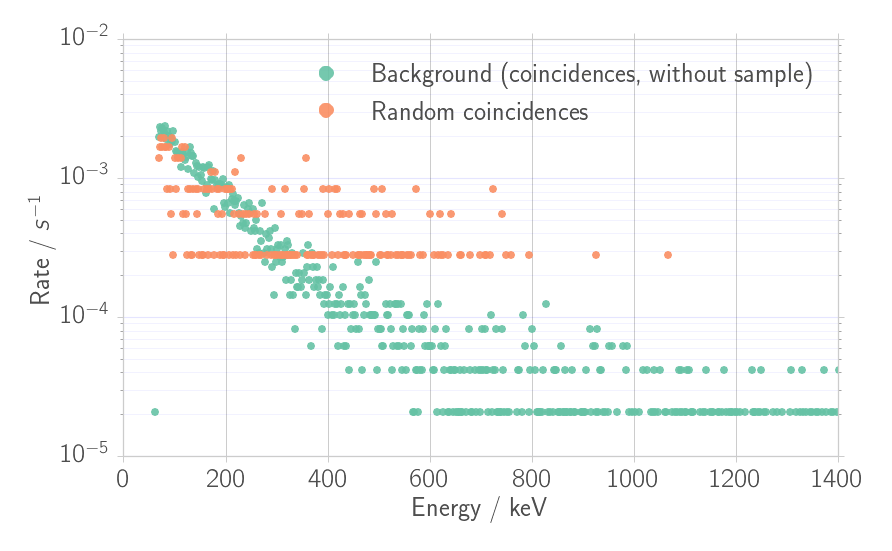
\includegraphics[width=1.0\linewidth]{../analysis/figures/coin_background_random}
    \label{fig:coin_ps_background}
\end{figure}

\end{frame}

\begin{frame}[t]{Energy of electrons: Rate of coincident events of PS scintillator at angle of $\theta = 90^\circ$}

    \begin{figure}[htpb]
    \centering
    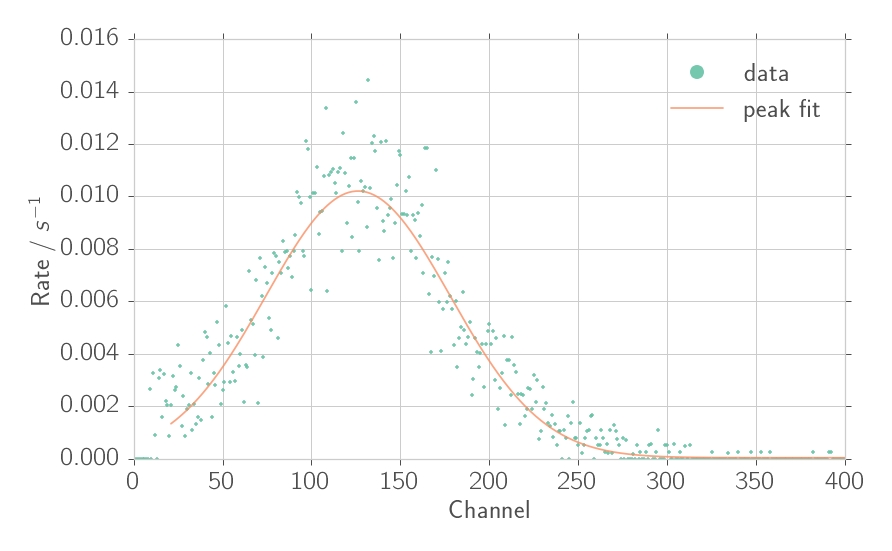
\includegraphics[width=1.0\linewidth]{../analysis/figures/coin_ps_90}
\label{fig:coin_ps_90}
\end{figure}

\end{frame}
\begin{frame}[t]{Energy of electrons: Rate of coincident events of PS scintillator at angle of $\theta = 15^\circ$}
    \begin{figure}[htpb]
    \centering
    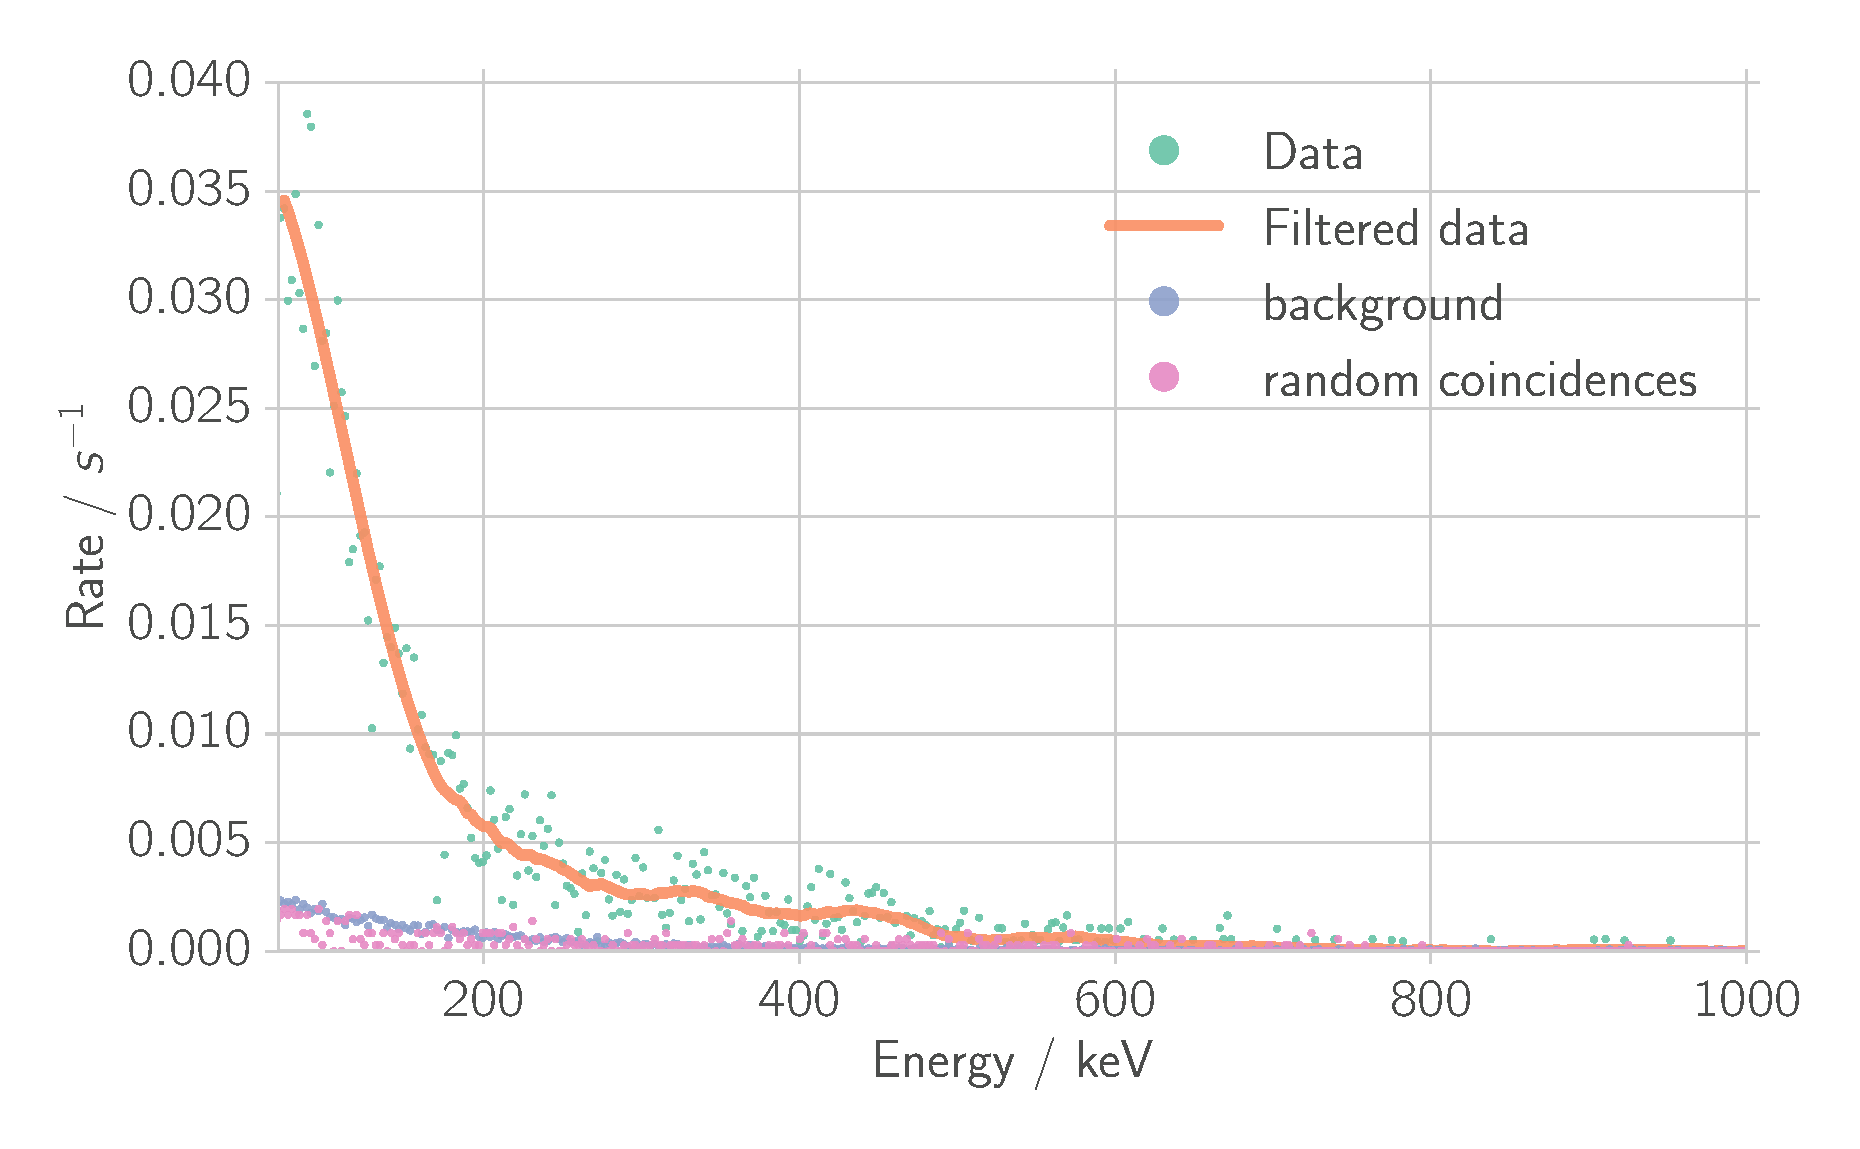
\includegraphics[width=1.0\linewidth]{../analysis/figures/coin_ps_15_filter_}
\label{fig:coin_ps_15}
\end{figure}
\end{frame}

\begin{frame}[t]{Background of NaI scintillator with coincidences (measurem. time 62h)}
   
\begin{figure}[htpb]
    \centering
    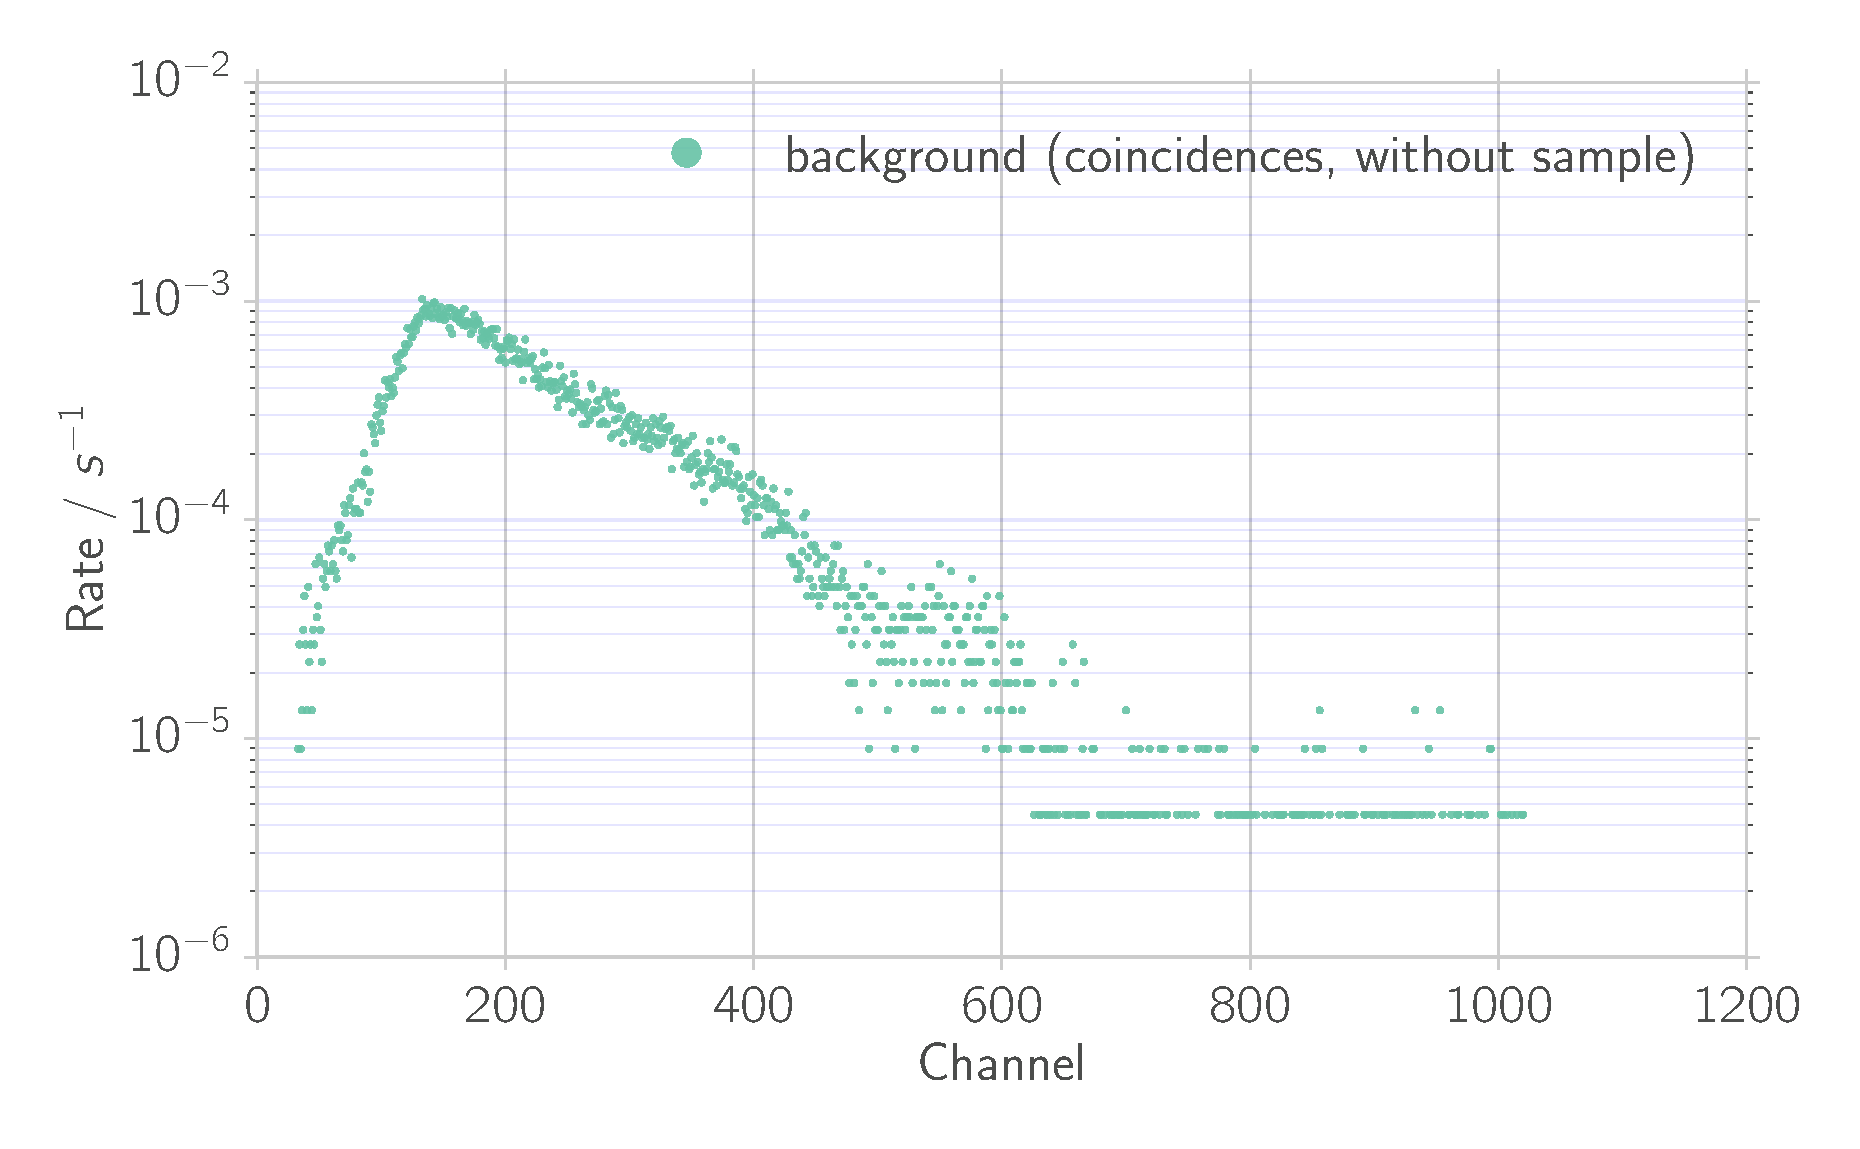
\includegraphics[width=1.0\linewidth]{../analysis/figures/coin_na_background}
\end{figure}
 
\end{frame}

\begin{frame}[t]{Energy of photons: Rate of coincident events of NaI scintillator at angle $\theta = 30^\circ$}
\begin{figure}[htpb]
    \centering
    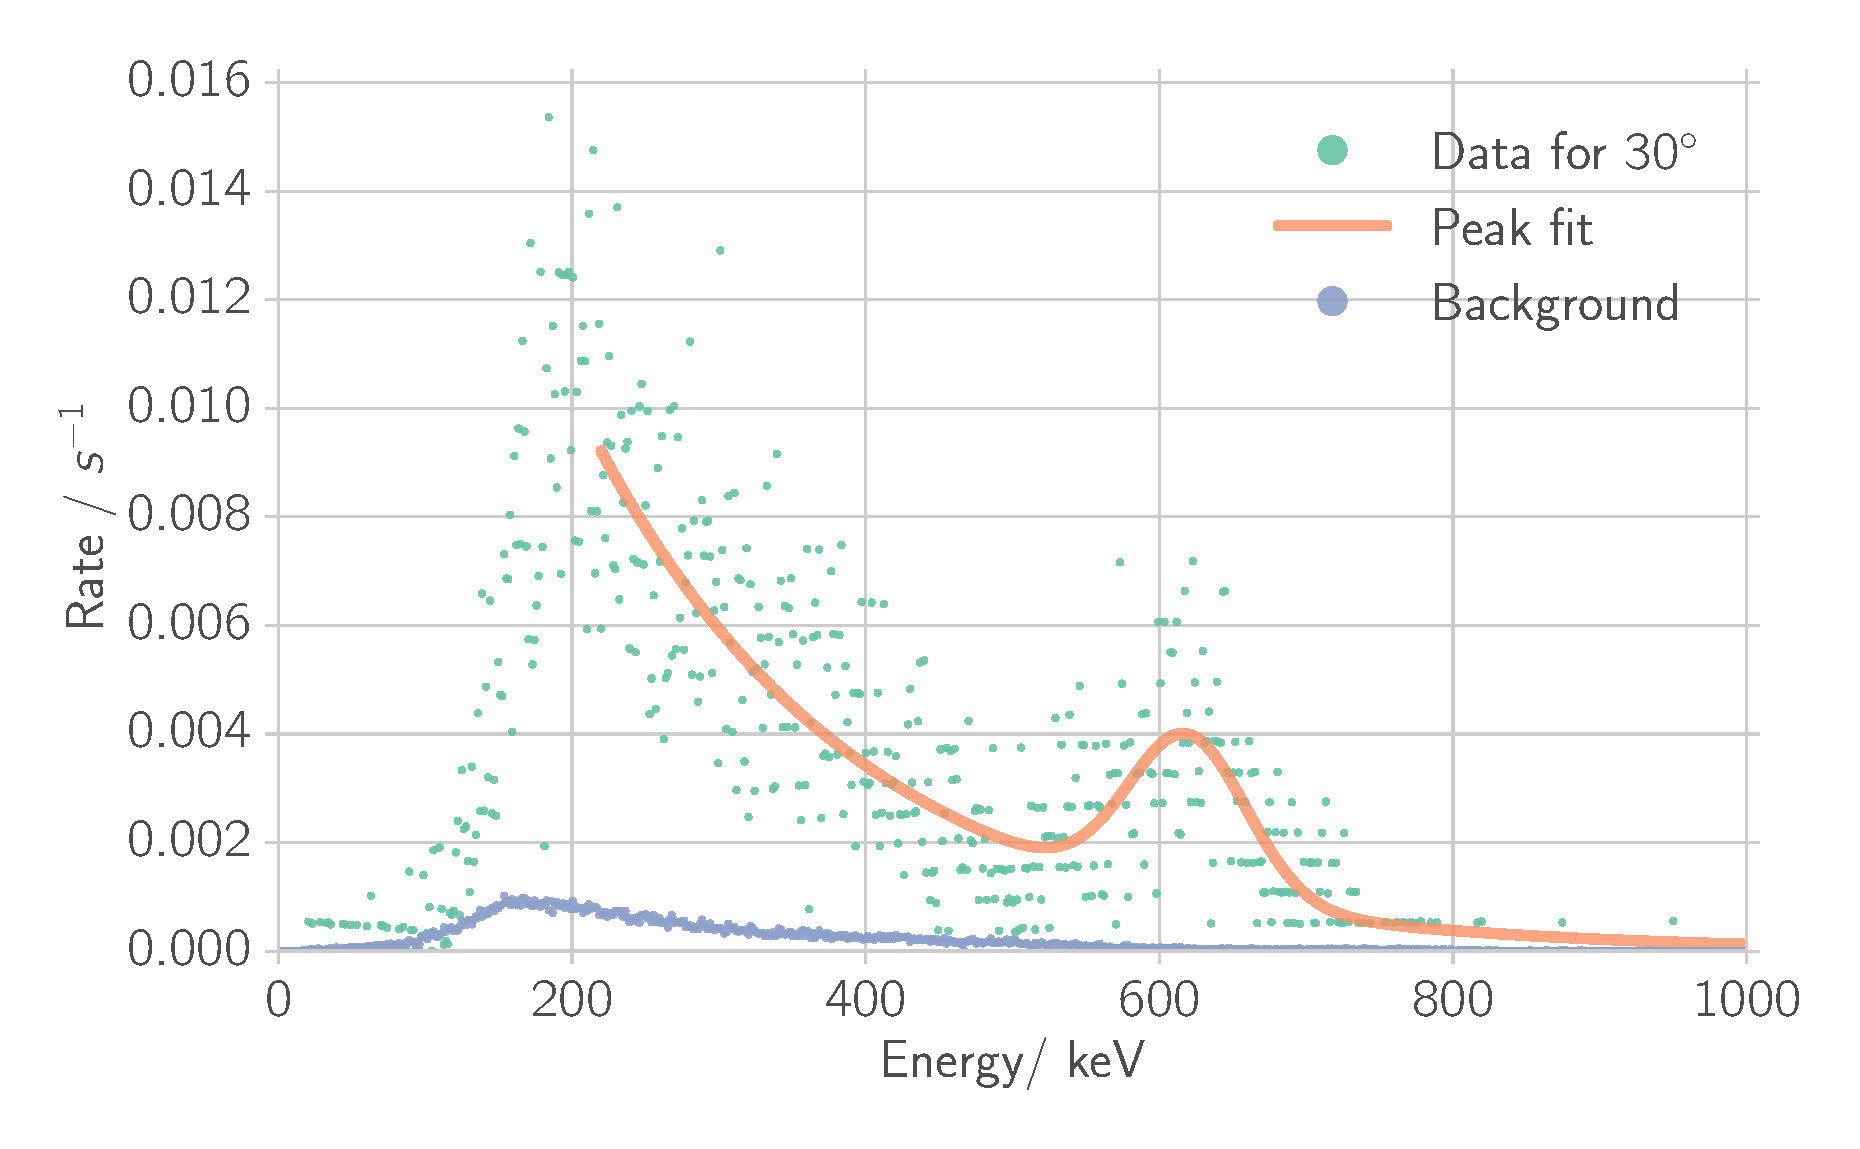
\includegraphics[width=1.0\linewidth]{../analysis/figures/coin_na_30}
    \label{fig:coin_na_30}
\end{figure}
\end{frame}

\begin{frame}[t]{Energy of photons: Rate of coincident events of NaI scintillator at angle $\theta = 90^\circ$}
\begin{figure}[htpb]
    \centering
    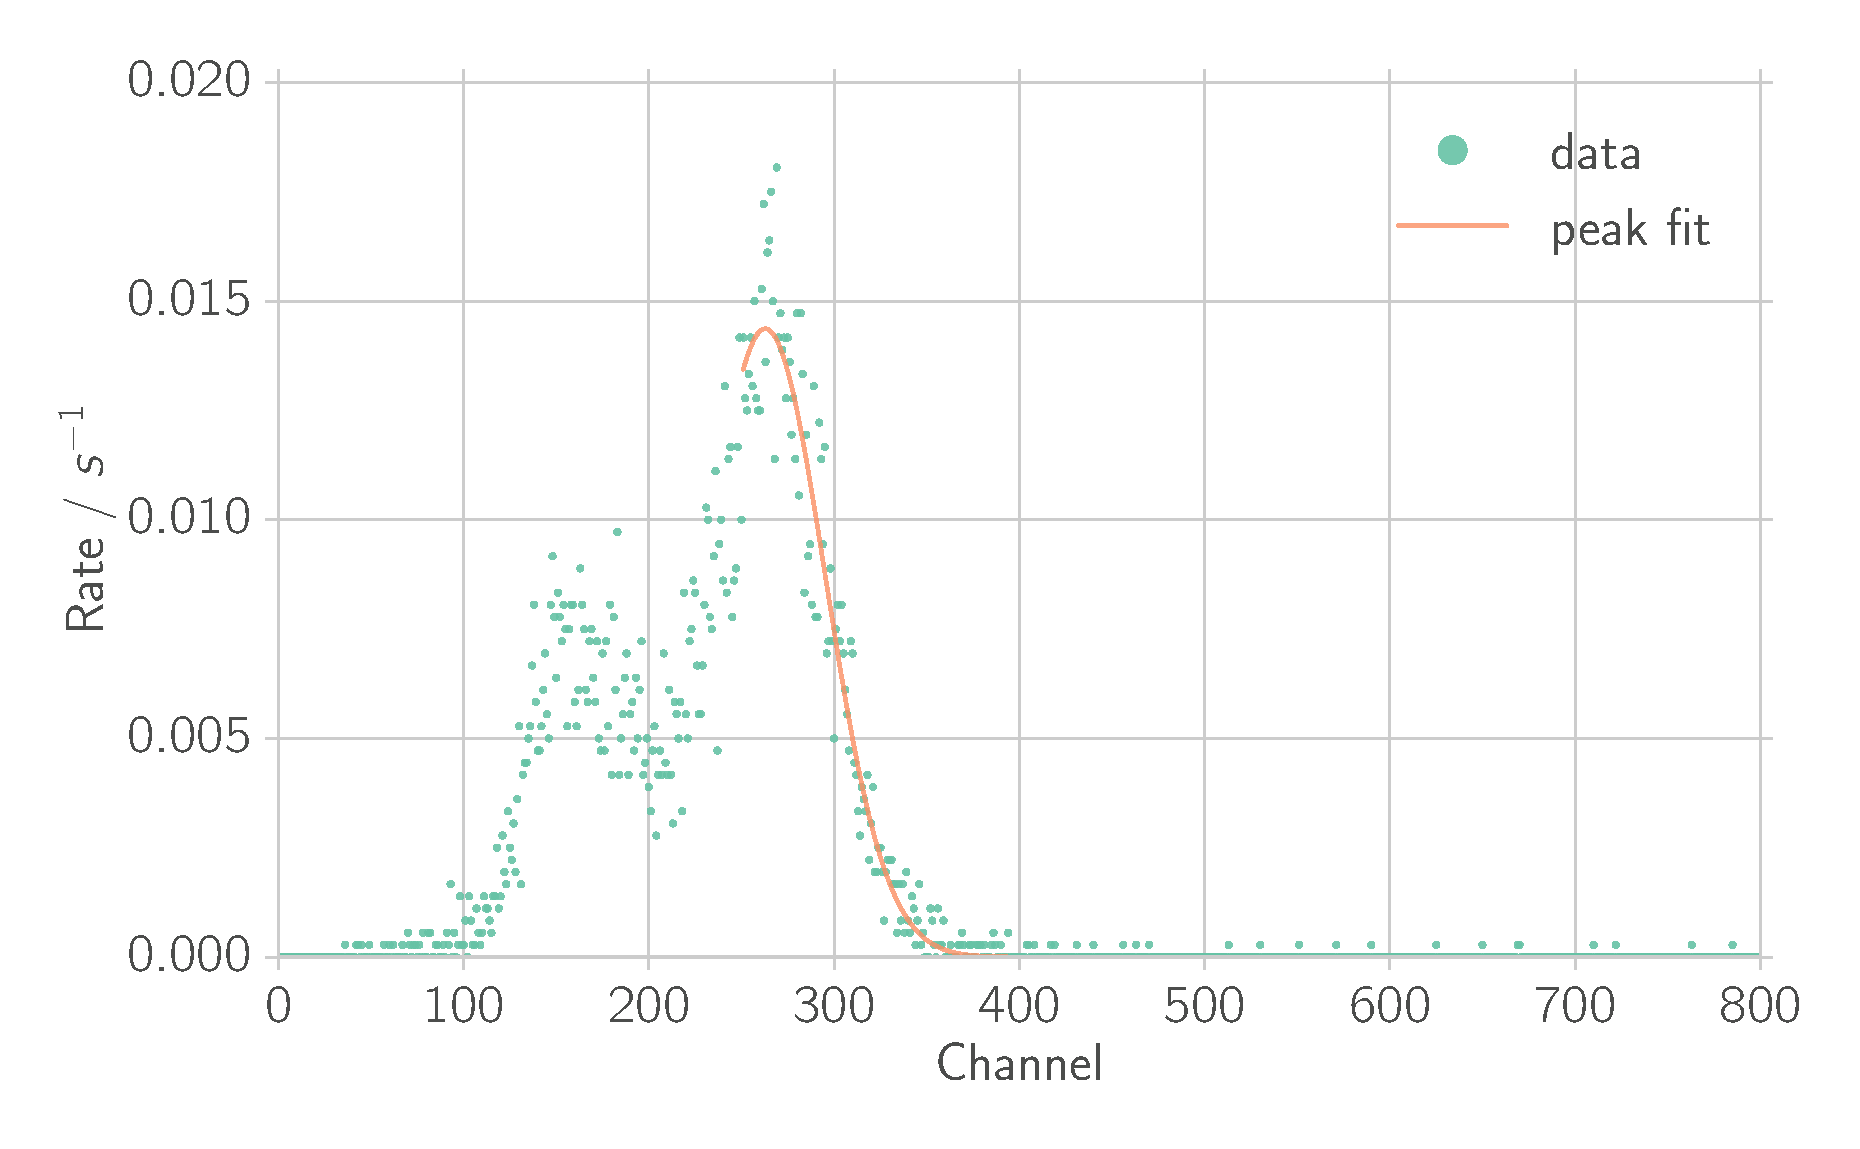
\includegraphics[width=1.0\linewidth]{../analysis/figures/coin_na_90}
    \label{fig:coin_na_30}
\end{figure}
\end{frame}

\begin{frame}[c]{}
    Now to the result: combining all those peaks...
\end{frame}


\end{document}
